\subsection{$90\degree$ Turn}

\subsubsection{Curved $90\degree$ Turn}

Figures \ref{fig:turns_cur_90deg_pos} and \ref{fig:turns_cur_90deg_camera} shows the optimized paths of a curved $90\degree$ turn with varying radii. The results show that with a radius of $200$m, $150$m, and $50$m the optimization algorithm returns a smooth stable flight path. As expected the camera position deviates more from the ground path than for gentler turns, and Figure \ref{fig:turns_cur_90deg_roll} shows that the roll angles contains some smaller spikes that did not appear in the $70\degree$ turn.

For all the three radii there is a deviation between the camera centre point and the ground path after the turn. For the $50$m radius turn in Figure \ref{fig:turns_cur_90deg_camera_50}, this deviation is as high as $50$m. While this most likely would correct itself of the path was simulated further, the deviation is a result of how the cost function is weighted. As mentioned in the previous section the weight on the camera position is so low compared to the weight put on the control rates, so having a deviation is cheaper than using control input to correct it.

A more surprising result is seen in Figures \ref{fig:turns_cur_90deg_position_100} and \ref{fig:turns_cur_90deg_camera_100}. Even though the MPC is able to optimize the turn with $50$m radius, it is not able to return a stable flight path for the turn with $100$m radius. As for the linear $70\degree$ corner, the MPC appears to fail mid-turn, which causes the aircraft to enter a spiral motion. As the MPC handles the other radii well, this may occur because of a very unfortunate set of waypoints, as mentioned for the failing horizon length.

\begin{figure}
	\makebox[\textwidth][c]{
	\subfloat[$200$m][$200$m]{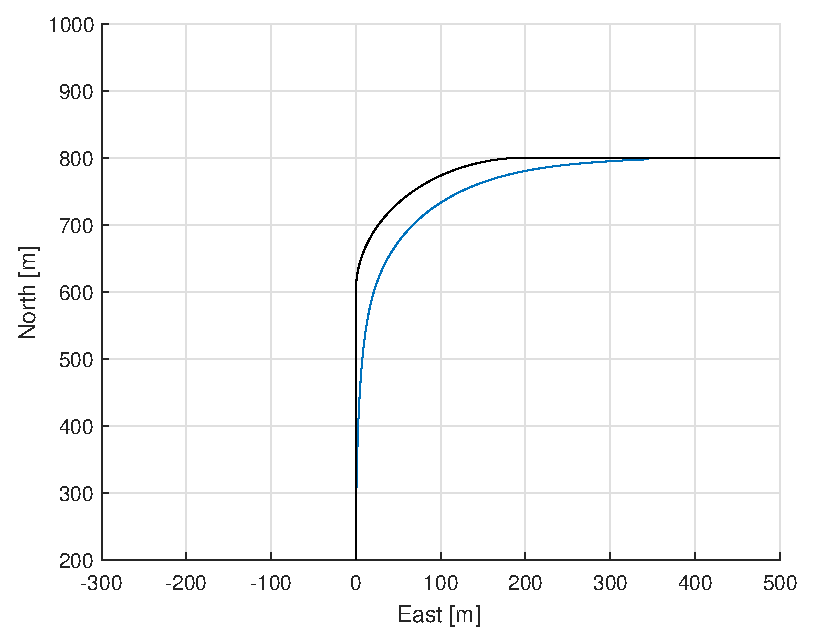
\includegraphics[width=0.5\textwidth, keepaspectratio=true]{../../results/opt/turns/curved/fig_90deg/uav_position_200m.eps}}
	\qquad
	\subfloat[$150$m][$150$m]{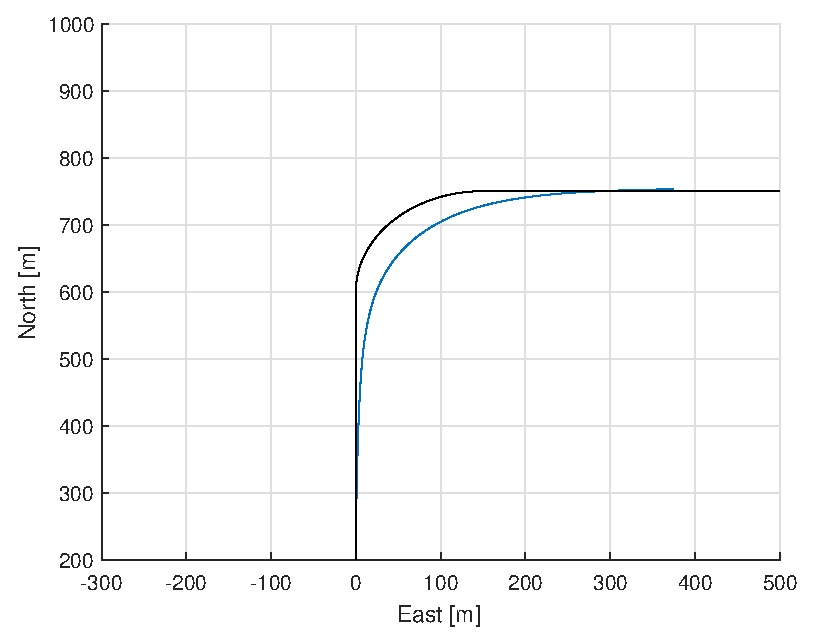
\includegraphics[width=0.5\textwidth, keepaspectratio=true]{../../results/opt/turns/curved/fig_90deg/uav_position_150m.eps}}}
	\makebox[\textwidth][c]{
	\subfloat[$100$m][$100$m]{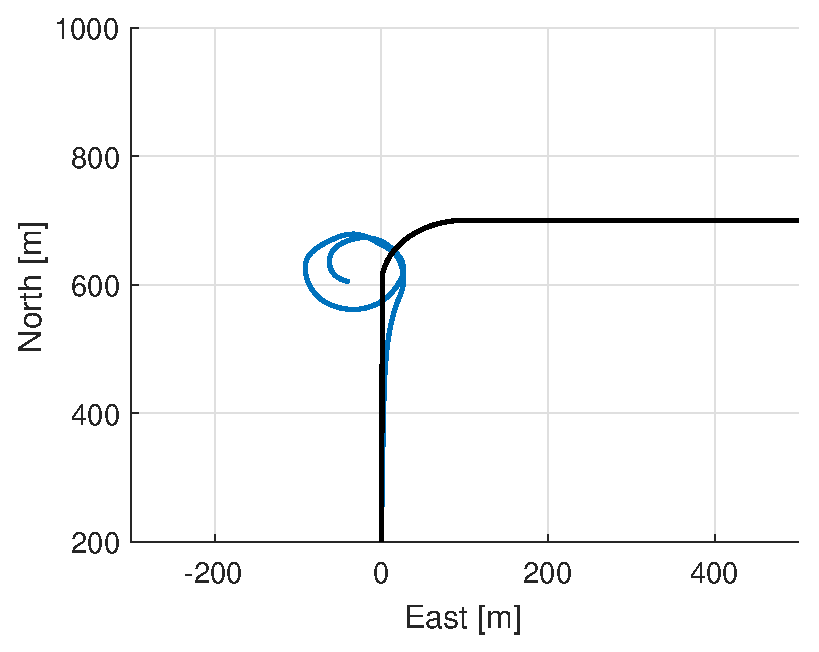
\includegraphics[width=0.5\textwidth, keepaspectratio=true]{../../results/opt/turns/curved/fig_90deg/uav_position_100m.eps}
	\label{fig:turns_cur_90deg_position_100}}
	\qquad
	\subfloat[$50$m][$50$m]{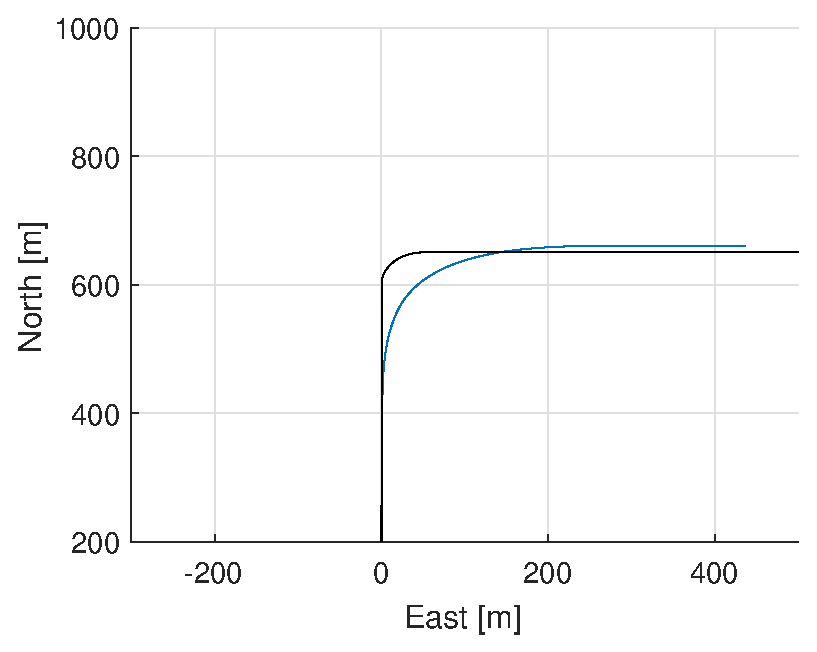
\includegraphics[width=0.5\textwidth, keepaspectratio=true]{../../results/opt/turns/curved/fig_90deg/uav_position_50m.eps}}}
	\caption{The position of the UAV when optimizing a curved $90\degree$ turn with varying radius.}
	\label{fig:turns_cur_90deg_pos}
\end{figure}

\begin{figure}
	\makebox[\textwidth][c]{
	\subfloat[$200$m][$200$m]{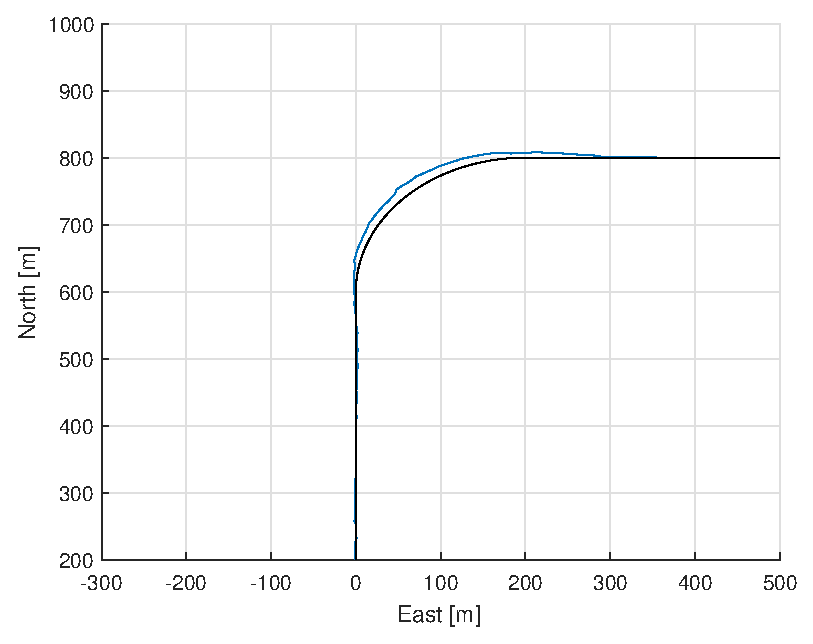
\includegraphics[width=0.5\textwidth, keepaspectratio=true]{../../results/opt/turns/curved/fig_90deg/camera_position_200m.eps}}
	\qquad
	\subfloat[$150$m][$150$m]{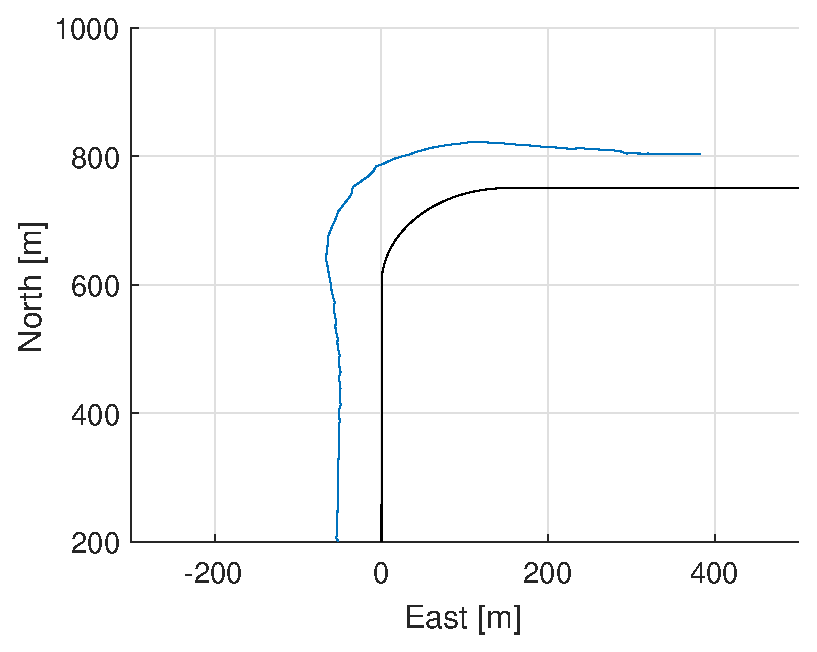
\includegraphics[width=0.5\textwidth, keepaspectratio=true]{../../results/opt/turns/curved/fig_90deg/camera_position_150m.eps}}}
	\makebox[\textwidth][c]{
	\subfloat[$100$m][$100$m]{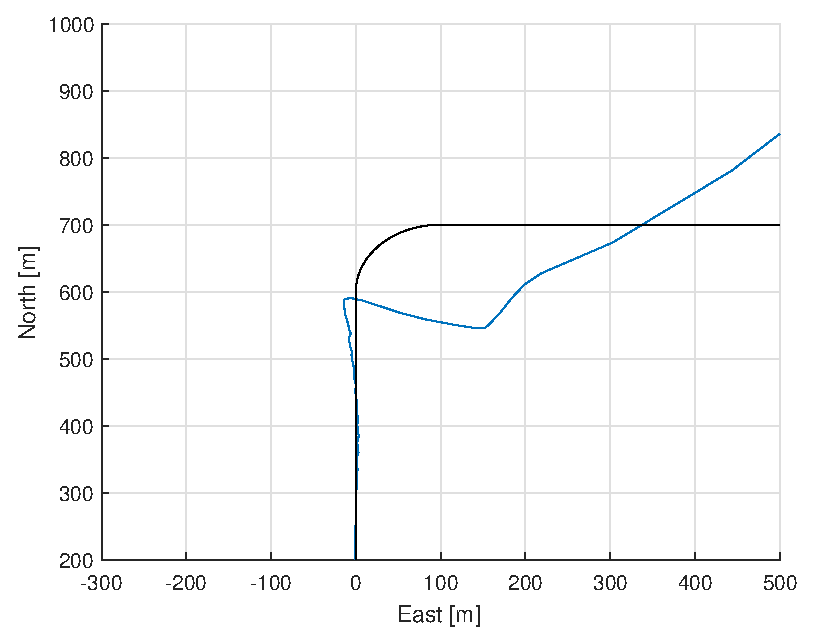
\includegraphics[width=0.5\textwidth, keepaspectratio=true]{../../results/opt/turns/curved/fig_90deg/camera_position_100m.eps}
	\label{fig:turns_cur_90deg_camera_100}}
	\qquad
	\subfloat[$50$m][$50$m]{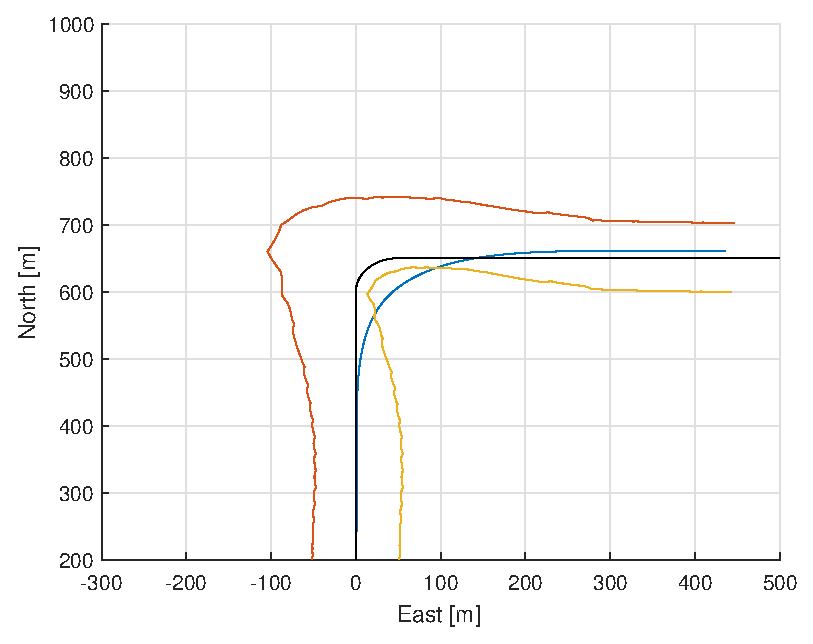
\includegraphics[width=0.5\textwidth, keepaspectratio=true]{../../results/opt/turns/curved/fig_90deg/camera_position_50m.eps}
	\label{fig:turns_cur_90deg_camera_50}}}
	\caption{The position of the camera when optimizing a curved $90\degree$ turn with varying radius.}
	\label{fig:turns_cur_90deg_camera}
\end{figure}

\begin{figure}
	\makebox[\textwidth][c]{
	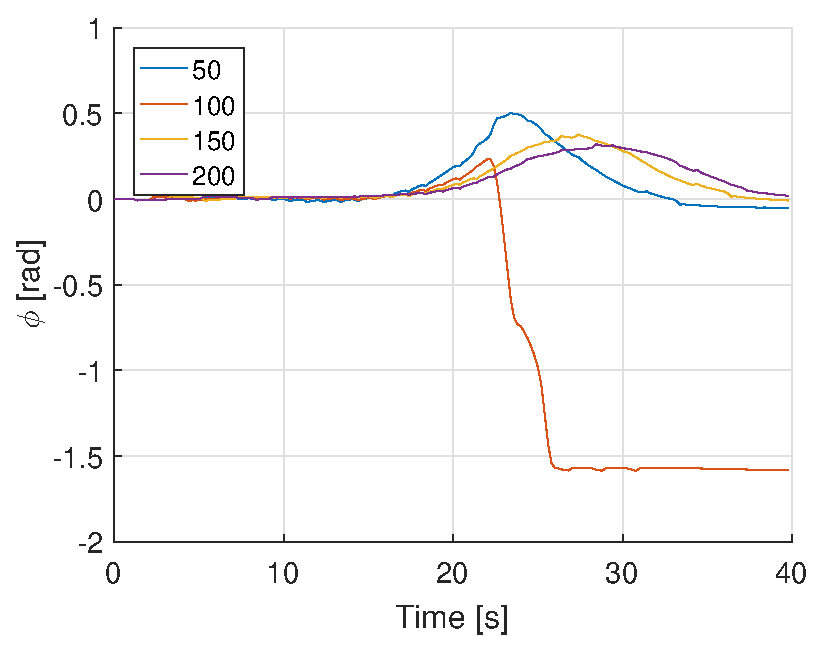
\includegraphics[width=0.8\textwidth, keepaspectratio=true]{../../results/opt/turns/curved/fig_90deg/attitude.eps}}
	\caption{The roll angle $\phi$ during the $90\degree$ turns.}
	\label{fig:turns_cur_90deg_roll}
\end{figure}


\subsubsection{Linear $90\degree$ Turn}

Since the MPC struggles to track a $70\degree$ corner, it is no surprise that it fails to track a $90\degree$ corner as seen in Figure \ref{fig:turns_lin_90deg}. Once again the MPC ends up with solving a difficult path using roll instead of the position, which ends with a bad solution. Different weightings on the position was tested without success.

\begin{figure}
	\makebox[\textwidth][c]{
	\subfloat[UAV position][UAV position.]{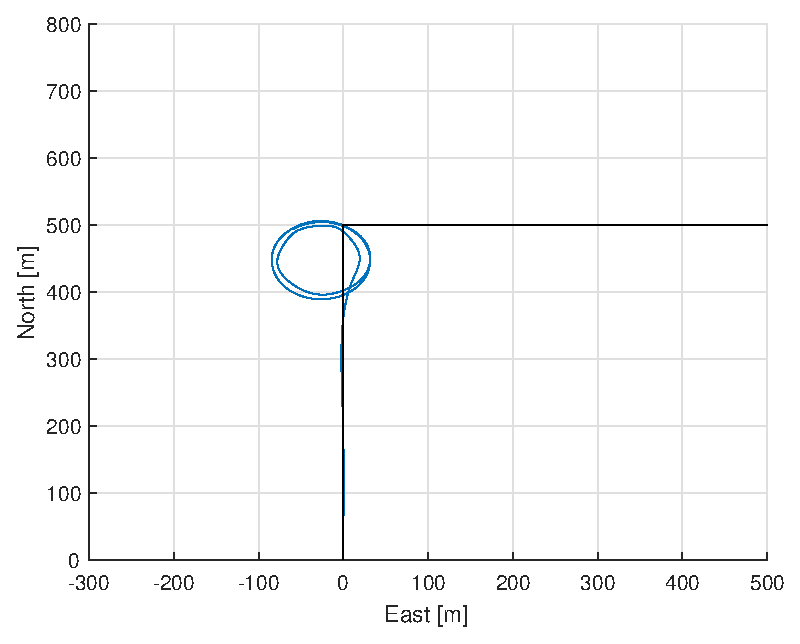
\includegraphics[width=0.5\textwidth, keepaspectratio=true]{../../results/opt/turns/linear/fig_90deg/uav_position.eps}}
	\qquad
	\subfloat[Camera position][Camera poistion.]{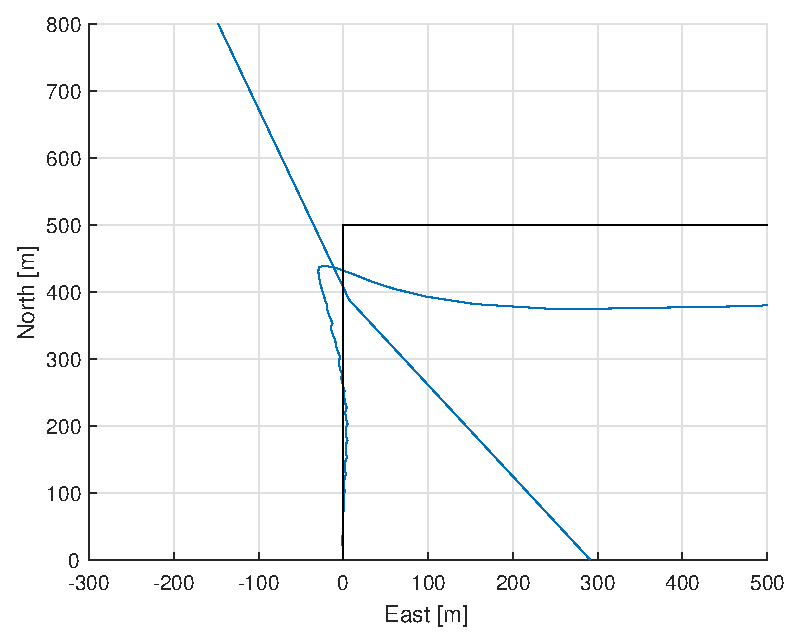
\includegraphics[width=0.5\textwidth, keepaspectratio=true]{../../results/opt/turns/linear/fig_90deg/camera_position.eps}}}
	\caption{Result of attempting to optimize a linear $90\degree$ turn.}
	\label{fig:turns_lin_90deg}
\end{figure}